%\section{Extensions of \trip}

\subsection{Personalized Constraints}
\label{sec:personalized}

We next the basic ILP problem, outlined in Eq.~\eqref{eq:max}--Eq.~\eqref{eq:self} to personalized constraints.

\subsubsection{Must-visit POIs}
\label{sec:must}

Suppose the traveler specifies a list of POIs $[m_1, \dots, m_k]$ that she
must visit.  Simply enforcing the corresponding $y$ binary variables to
$1$ ensures that these POIs are chosen in the optimal itinerary:
%
\begin{align}
	\label{eq:see}
	y_{m_i} & = 1, \forall i = 1, \dots, k
\end{align}

\subsubsection{Must-avoid POIs}
\label{sec:avoid}

Similarly, if the traveler explicitly lists a set of POIs $[a_1, \dots,
a_k]$ that she does not want to visit, the corresponding $y$ binary
variables are simply set to $0$:
%
\begin{align}
	\label{eq:avoid}
	y_{a_i} & = 0, \forall i = 1, \dots, k
\end{align}

\subsubsection{Category Constraints}
\label{sec:category}

To handle category contraints where a traveler specifies the range of
number of POIs that she wants to visit for a category, we augment the
variable $y$ associated with every POI with a category superscript.  For
example, if there are $l$ categories, the corresponding variables $y^1,
\dots, y^l$ represent the different possibilities.  If POI $i$ belongs to
category $k$, then, by definition, $y^j_i = 0, \forall j \neq k$, for
every other category $j$.  If every category $k$ has a lower bound $lb^k$
and upper bound $ub^k$ on number of POIs to be visited, then the basic
problem can be augmented by:
%
\begin{align}
	\label{eq:category}
	lb^k \leq \sum_{\forall i} y^k_i & \leq ub^k, \forall k
\end{align}
%
If the traveler only specifies the minimum number of POIs of a category
$k$ that she must visit, the upper bound $ub^k = N$; similarly, specifying
only the maximum number puts the lower bound as $lb^k = 0$.  For
categories where no constraint is mentioned, $lb^k = 0$ and $ub^k = N$.

\subsubsection{Ordering Constraints}
\label{sec:ordering}

A traveler can impose an ordering constraint, where she states that she will
visit POI $j$ before POI $k$, if the itinerary contains both of them.
To impose these ordering constraints, we introduce a \emph{start time} value for each POI, denoted by $s_i$ for node $v_i$.
If POI $j$ must be visited before POI $k$ (denoted as $j \prec k$), then $s_k$ must be after $s_j$ plus
the time it takes to visit $v_j$ (i.e., $t_{v_j}$) and the time it takes to
reach $v_k$ from $v_j$ (i.e., $t_{v_j,v_k}$).
Hence,
%
\begin{align}
	s_j + t_{j} + t_{j,k} & \leq s_k, \forall j \prec k
\end{align}
%
The above equation assumes that both POIs $j$ and $k$ are vsiited.
However, it may be the case that either $j$ or $k$ or both is not visited at all.
To handle the case that $j$ is not visited, the lower bound of $s_j$ for any
node is kept as $0$, and the times are added only if $y_j = 1$.
To handle the case that $k$ is not visited, a large value $M$ is added to $s_k$
when $y_k = 0$.
Together, the ordering constraint equation becomes
%
\begin{align}
	\label{eq:ordering}
	s_j + (t_{j} + t_{j,k}) \cdot y_j & \leq s_k + M \cdot (1 - y_k), \forall j \prec k
\end{align}

\subsection{POI Timings}
\label{sec:timings}

Many POIs have certain operating times.  For example, a temple may be open
only in the morning, from 9-11am.  Even otherwise, a traveler may specify that she wants to visit the temple in the morning hours only.  To handle this constraint, the start and
end time of the POI must be within this operational time.  Hence, if a POI
$i$ has an operational time denoted by entry and exit times $[en_i, ex_i]$,
then
%
\begin{align}
	\label{eq:operational}
	s_i \geq en_i \text{ and } & s_i + t_{i} \leq ex_i
\end{align}

\ignore{
		
\begin{itemize}

\item \textbf{Must-see POIs}\\
This constraint enforces that each POI marked as a must-see is visited exactly once over the duration of the trip:

\begin{equation}
\label{mul_day_7}
    \sum_{d \in \text{days}} y_{i,d} = 1 \quad \quad \forall i \in \text{must\_see\_pois}
\end{equation}

where:
\begin{itemize}
  \item \texttt{must\_see\_pois} is the set of user-specified must-visit POIs
\end{itemize}
\item \textbf{Must-avoid POIs}\\
This constraint enforces that each POI marked as excluded is never visited in the entire trip:

\begin{equation}
\label{mul_day_8}
    \sum_{d \in \text{days}} y_{i,d} = 0 \quad \quad \forall i \in \text{excluded\_pois}
\end{equation}

where:
\begin{itemize}
  \item \texttt{excluded\_pois} is the set of user-specified excluded POIs
\end{itemize}
\item \textbf{Category Constraints}\\
The user can specify the lower bound and upper bound for the categories of POIs to be visited across the trip. This constraint ensures that user's preferences over these themes are respected:

\begin{align}
\label{mul_day_11}
lb_m \leq \sum_{i \in V_m} \sum_{d \in \text{days}} y_{i,d} \leq ub_m, \quad \forall m \in C 
\end{align}

where:
\begin{itemize}
  \item \( C \) represents all the categories (e.g., historical, cultural, adventure, etc.)
  \item \( lb_m \) and \( ub_m \) are the lower and upper bounds for theme \( m \)
\end{itemize}

\item \textbf{Ordering Constraints}\\
If (a,b) is an ordering constraint, then POI a and POI b can be visited on different days, so this constraint makes sure that day of visit of POI a is before, or same as day of visit of POI b.
\begin{align}
\label{mul_day_12}
\texttt{day\_visit}_a \leq \texttt{day\_visit}_b, \quad \forall (v_a, v_b) \in P
\end{align}
\noindent
where:
\begin{itemize}
    \item \( \texttt{day\_visit}_a \): the day on which POI \( a \) is visited.
    \item \( P \): the set of all ordered POI pairs with ordering constraints entered by the tourist.
\end{itemize}

\item

\textbf{2. Intra-day Temporal Ordering Constraint}\\
If (a,b) is an ordering constraint and both POI a and POI b are to be visited on same day, then this constraint ensures that arrival time of POI b is greater than or equal to sum of arrival time of POI a, visit duration of POI a and travel time from POI a to POI b.

\begin{align}
\label{mul_day_13}
s_{i,d} + \left( t(v_i) + \left( t^{w}_{i,j} \cdot w_{i,j,d} + t^{t}_{i,j} \cdot x_{i,j,d} \right) \right) y_{i,d}
&\leq s_{j,d} + T_{ij} (1 - y_{j,d})\\ \forall (v_i, v_j) \in P,\; \forall d \in \text{days} \nonumber \\
\label{mul_day_14}
T_{ij} = ct(v_i) + t(v_i) + t^{w}_{i,j} 
\end{align}

\noindent
where:
\begin{itemize}
    \item \( s_{i,d} \): start time of visiting POI \( i \) on day \( d \).
    \item \( t(v_i) \):visit time spent at POI \( i \).
    \item \( ct(v_i) \): closing time of POI \(v_i\) \( i \).
\end{itemize}

\noindent
The Big-M term \( T_{ij} (1 - y_{j,d}) \) ensures the constraint becomes non-restrictive when POI \( j \) is not selected on day \( d \).
\end{itemize}

}

\subsection{Utility Variants}
\label{sec:utility}

The basic problem formulation assumes a traveler visits a POI for a fixed amount
of time, and gets the full utility offered by the POI.  However, in real life,
the time spent by every traveler is not the same.  Some may finish visiting a
POI in lesser time than the prescribed one, while some others may take longer
time.  In addition, some may not be willing to spend the full time in a POI, and
may sacrifice getting the full utility for partial utilization, and may come out
early to save time, and visit other POIs.  For example, a museum may have many
different types of rooms, such as sculpture, paintings, jewelry, etc., and a
traveler may not like to visit the jewelry section.  She may, thus, decide to
spend only a part of the total visit time for the other sections, get a partial
utility, and exit to go to another POI.  To capture this, we model the utility
in three variants, as described next.

Note that in all of these variants, if a traveler spends \emph{more} time
than the prescribed time of visit, her utility is capped to 100\% only.

\subsubsection{Binary}
\label{sec:binary}

This is the standard utlity variant, where a traveler spends full time in a
POI, and gets the complete utility.  If she does not spend that time, she
gets no utility at all.

The binary utility $U^b_i$ of a POI $i$ for the binary variant is captured
simply by
%
\begin{align}
	\label{eq:binary}
	U^b_i & = U_i, \forall i
\end{align}

\subsubsection{Slab}
\label{sec:slab}

The binary utility variant is too strict, and does not allow any leeway.
In the slab utility variant, the total visit time is divided into various slabs, starting from
50\%.  (We assume that a POI must be visited for at least 50\% of its time
to get any utility.) Each \emph{slab} is an interval of time spent as a percentage
of the total visit time.  When a traveler spends time in a slab of
interval, she gets a percentage of utility equal to the lower end of the
interval.  Thus, if a slab is [60-70)\%, and a traveler spends 67\% time,
she gets a utility equal to 60\% of the total utility.

The utility value is divided into the same number of slabs as the visit
time.  In this paper, we divide into 6 slabs: [50-60), [60-70), [70-80),
[80-90), [90-100), [100-$\infty$), although this can be altered.
Correspondingly, we have 6 binary \emph{slab variables} for every POI,
$u^1, \dots, u^6$, with the constraint that at most one of them is chosen
(using the condition $\sum_{l=1}^6 u^l_i \leq 1$).  The \emph{effective
utility} of a POI $i$ is then:
%
\begin{align}
	\label{eq:slab}
	U^s_i = U_i \cdot ( & 0.5 \times u^1_i + 0.6 \times u^2_i + 0.7 \times u^3_i \nonumber \\
		& + 0.8 \times u^4_i + 0.9 \times u^5_i + 1.0 \times u^6_i )
\end{align}

\subsubsection{Continuous}
\label{sec:continuous}

The third variant models the utility as a continuous function equal to the
percentage of time spent.  (Again, we impose the minimum time to be spent
as 50\% for non-zero utility.) Thus, if a traveler spends 67\% time, she
gets 67\% utility.

The continuous variant introduces a variable $f_i$ to denote the fraction of utility got from a POI, corresponding to the time spent there.
Its upper and lower bounds are set to 1.0 and 0.5 respectively in the following manner:
%
\begin{align}
	\label{eq:fbound1}
	f_i & \geq 0.5 \cdot y_i \\
	\label{eq:fbound2}
	f_i & \leq y_i \\
	\label{eq:ybound1}
	f_i & \leq (0.5 - \epsilon) + y_i \\
	\label{eq:ybound2}
	f_i & \geq (0.5 - \epsilon) - (1 - y_i)
\end{align}
%
Eq.~\eqref{eq:fbound1} and Eq.~\eqref{eq:fbound2} put the bounds on $f_i$.
Eq.~\eqref{eq:ybound1} ensures that if $f_i \geq 0.5$, then $y_i = 1$,
i.e., the POI must be chosen.  Eq.~\eqref{eq:ybound2} ensures that if $f_i
< 0.5$, then $y_i = 0$, i.e., the POI must not be chosen.  ($\epsilon$ is a
tiny positive constant.)

The utility $U^c_i$ is then simply
%
\begin{align}
	\label{eq:continuous}
	U^c_i = U_i \cdot f_i
\end{align}

\ignore{

\noindent \textbf{Fractional Visits to POIs}\\
This feature enables partial visiting of Points of Interest (POIs), thus enhancing the flexibility and potential utility of the proposed itineraries. In comparison to the Binary approach used before which required the POI to be completely visited in order to collect its utility, the Fractional version built here grants proportional utility based on the proportion visited of the POI—improving time and cost budget efficiency.

\textbf{Fractional POI Variable (ppoi[i])}
\begin{itemize}
    \item A real variable $\text{ppoi}[i] \in [0, 1]$ is defined for every POI i to reflect the portion of the POI's total visit time covered by the itinerary.

    \item A threshold of 0.5 (50\%) is enforced: POIs must be visited for at least half of their average duration to be included. If ppoi[i] < 0.5, it is effectively set to 0 and the POI is excluded from the plan.
\end{itemize}

\textbf{Utility Calculation Variants}
\label{Utility_Calculation}

Two distinct methods are used to compute the utility in the fractional setting:

\begin{itemize}
\item {Continuous Linear Utility Model}

In this version, the utility granted is directly proportional to the fraction of the POI visited.

If a POI has utility $U$ and is visited for $p$ fraction of time (where $p \in [0.5, 1]$), the utility granted is $U \times p$.

\item{Slab-Based Utility Model}
\begin{itemize}[noitemsep, topsep=0pt]
    \item Fraction $\in$ [0.5, 0.6) $\rightarrow$ 50\% utility
    \item Fraction $\in$ [0.6, 0.7) $\rightarrow$ 60\% utility
    \item Fraction $\in$ [0.7, 0.8) $\rightarrow$ 70\% utility
    \item Fraction $\in$ [0.8, 0.9) $\rightarrow$ 80\% utility
    \item Fraction $\in$ [0.9, 1.0) $\rightarrow$ 90\% utility
    \item Fraction = 1.0 $\rightarrow$ 100\% utility
\end{itemize}

It is important to note that we provide 100\% utility if and only if POI is visited completely. The utility granted coincides with the lower bound because we do not want a situation like this to occur where even if we suggest that tourist visit 50\% POI and they get any utility greater than 50\% because that would scale up the actual utility as compared to the continuous linear function.
\end{itemize}

To enable fractional visits, the constraints were modified to make the visit duration at one POI proportional to a continuous variable \( ppoi_i \in [0,1] \), that represents the relative fraction of the overall visit duration spent at the POI \( v_i \). Accordingly, in all the constraints, the original visit times are multiplied by this fractional variable \( ppoi_i \), ensuring the constraints accurately reflect partial visits.

When the utility function is a continuous linear function of visit time, the utility score obtained from a POI is also scaled proportionally, i.e., \( \text{utility}_i = U(v_i) \cdot ppoi_i \), where \( U(v_i) \) is the full utility for a complete visit to POI \( v_i \).

For the slab-based utility variant, a continuous variable \( \text{effective\_utility}_i \) is used to capture the actual utility awarded based on the fraction of time spent at each POI. The utility is determined using discrete slab multipliers based on the visit duration. Each POI is assigned to at most one slab, and the utility is calculated as:

\begin{align}
\label{effective_utility}
\text{effective\_utility}_i &= U(v_i) \cdot \big(0.5 \cdot s_1[i] + 0.6 \cdot s_2[i] + 0.7 \cdot s_3[i] \notag \\
&\quad + 0.8 \cdot s_4[i] + 0.9 \cdot s_5[i] + 1.0 \cdot s_6[i] \big)
\end{align}

The optimization objective is to maximize the total utility accumulated across all POIs:

\begin{align}
\label{objective_fun_slabs}
U(I) = \sum_{i=1}^N \text{effective\_utility}_i
\end{align}

To ensure only one slab level is chosen per POI, the following constraint is imposed:

\begin{align}
\sum_{k=1}^{6} s_k[i] \leq 1, \quad \forall i \in \{1, \dots, N\}
\end{align}

}

\subsection{Multi-Day Itinerary}
\label{sec:multiday}

For large tourist-forendly cities, covering all the POIs may not be
possible within a single day, and travelers typically look for
\emph{multi-day} tour itineraries.  Most work solve it trivially by first
running for a single-day, getting rid of the POIs covered in that day, and
then running again for the next day, and so on.  Instead, we solve the
problem as one single optimization problem.  For each day, we can specify a
source and destination, and the time budget.  This caters to tours where
the time in the first and last days are typically less due to arrival and
departure constraints.  Also, the first day's source and the last day's
destination may be an airport or a rail station, while for other days, it
is a hotel.

For an itinerary having $d$ days, we augment all the variables with a
superscript that indicates the day of the visit.  Thus, the $y$ and $z$
binary variables are replicated for each day: $y^d_i$ and $z^{m,d}_{j,k}$
for all POIs $i$, modes of transport $m$ and days of visit $d$.  While the
cost budget (Eq.~\eqref{eq:cost}) is imposed on the overall tour, the time
budget constraints (Eq.~\eqref{eq:time}) are imposed per day.  The rest of
the constraints--incoming, outgoing, mode, connectivity, nodechoice,
edgechoice, and no self loop--(Eq.~\eqref{eq:sout} to Eq.~\eqref{eq:self})
remain the same, and are applied for each day.  Additionally, the following
conditions ensure that a POI is chosen at most once within $d$ days:
%
\begin{align}
	\label{eq:multiday}
	\sum_{\forall d} y^d_i & \leq 1, \forall i
\end{align}
%
Choosing a POI at most once automatically constraints choosing any incoming
or outgoing edge to or from it to at most once as well.

\subsection{Dynamic Itinerary Re-planning}
\label{sec:dynamic}

So far, we have discussed only static plans.
Once an optimal tour is decided, it is not altered.
However, in real life, both tourist behavior as well as other conditions including weather, traffic, etc. are not deterministic in nature, and change over time.
To handle this, we introduce \emph{dynamic tour re-planning} where we keep computing the best tour given the current situation.
To the best of our knowledge, no other tour planner does that.

We initially start with an optimal static plan using our solver that takes into account the traveler's preferences.
However, after visit of every POI, we provide an option to her to \emph{re-optimize} the rest of the plan based on the current situation.
This may happen since she may have spent substantially less or more time in a POI, or the current traffic condition has somehow altered significantly due to accidents, etc.

Our solver now replans the schedule based on the remaining time and cost
budgets. The POIs already visited are not considered further (they are
added as must-avoid POIs), and the current POI is considered the source.
This optimizes the rest of the tour based on current progress and not
static assumptions.

\ignore{

The real tourist behavior and weather conditions, are dynamic and unpredictable in nature. They can be influenced by unforeseen delays, detours, longer-than-anticipated visits, or spontaneous user preferences, which can significantly impact the feasibility and correctness of an advanced preplanned itinerary. To close the gap between theory and practice, a dynamic approach is required.

In contrast with the static approach used in \cite{taylor2018tour}, where rigid, precomputed travel times and POI visit times, we have taken real-time travel times using Google-Maps API (Routes API). 

On the top of suggested times of visit and travel, user can enter the actual time they have taken to visit a POI and the travel time they took to reach the current POI.

With every visit to a POI, the system replans the schedule based on the remaining time and cost budgets. The POIs already visited are not considered for further itineraries. This optimizes the rest of the day based on current progress and not stale assumptions.

For the dynamic feature, a record of visited POIs was maintained. On visiting a POI, it was eliminated from the list to be taken into account in future itinerary calculations with the new remaining time and cost budgets.

}

\ignore{

\begin{figure}[th]
\textbf{Implementation of Dynamic Approach}
\centering
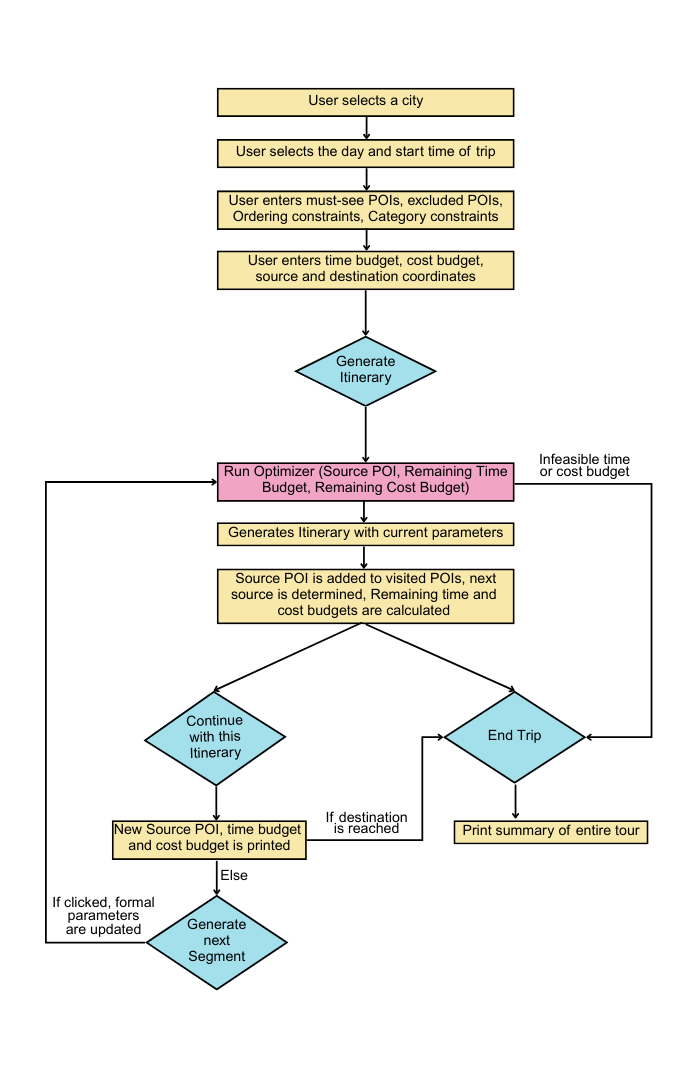
\includegraphics[width=0.5\textwidth]{binary dynamic flowchart.png}
	\caption{Implementation of Dynamic Approach -- \ab{is this figure needed? May be simplify}}
\label{fig:flowchart_dynamic}
\end{figure}

}

